%!TEX root = ../template.tex
%%%%%%%%%%%%%%%%%%%%%%%%%%%%%%%%%%%%%%%%%%%%%%%%%%%%%%%%%%%%%%%%%%%%
%% chapter5.tex
%% NOVA thesis document file
%%
%% Chapter with lots of dummy text
%%%%%%%%%%%%%%%%%%%%%%%%%%%%%%%%%%%%%%%%%%%%%%%%%%%%%%%%%%%%%%%%%%%%

\typeout{NT FILE chapter5.tex}%

\chapter{System Design and Realization}
\label{cha:impl}


\epigraph{ \textit{This chapter describes the technical implementation of the proposed configuration language for RAMSES. It details how the insights from industrial collaboration informed the architectural decisions and how each feature was implemented.}}


\section{Industry Partner Meeting}
\label{sec:industry_meeting}

The first meeting with an industry partner revealed to be very useful with many insights to note, particularly that a few features were highlighted and prioritized in order to maintain a good development speed and an overall better plan. Most of the previously thought of features (Identifiers, Traceability, Report, etc) were endorsed, however, a new feature was suggested by an expert \gls{ROS} developer: the separation of \gls{ROS} specific code and C++ specific code, meaning that code that is specific to \gls{ROS} can be isolated as it is very similar along the various generated files. This will essentially be done with an interface that will implement \gls{ROS} code on C++ only files, which effectively serves as a separation of concerns.

\begin{tcolorbox}[colback=green!5, colframe=green!40!black] This meeting provided extremely valuable insight as the industry partner has been using \gls{ROS} for over seven years, effectively distilling their experience into actionable knowledge. \end{tcolorbox}


\section{Implementation Plan} 
\label{sec:impl_plan}

In order to better understand what features will be implemented, when and why, the implementation will be done by layers, each layers will depend on things done previously on other layers, hence some features are developed before others.

\bgroup
\rowcolors{1}{}{GhostWhite}
\begin{xltabular}{\textwidth}{X X X}
	\caption{Feature dependency table}
	\label{tab:impl_plan}\\
	\toprule
	\rowcolor{Gainsboro}%
	Feature & Depends On & Notes \\
	\midrule
	Identifiers & – & Core to code structure \\
	Comments & Identifiers & Cheap to implement early \\
	Traceability & Identifiers, Comments & Hard to retrofit later \\
	Report & Traceability & Uses trace data \\
	Standard\par Compliance & Report, Traceability & Enforce compliance early \\
	Dead Code\par Elimination & Traceability, Report & Needs stable generation logic \\
	Memory\par Optimization & Dead Code Elim, Traceability & Impacts data structures directly \\
	Node Interface & Memory Optimization & Enables \gls{ROS} decoupling \\
	Legacy Code\par Integration & Node Interface & Most architecture-dependent \\
	\bottomrule
\end{xltabular}


Table~\ref{tab:impl_plan} presents the planned order of feature implementation based on their dependencies. Each feature may require elements developed in previous steps, ensuring a coherent and manageable progression. This dependency structure prevents rework by implementing features that provide necessary infrastructure before higher-level functionalities.


\subsection{Core and Metadata Layer}
\label{sec:code_and_meta}

The Core and Metadata Layer (Table~\ref{tab:core_and_meta}) includes foundational features that establish the basic code structure and metadata necessary for subsequent processing. Features such as identifiers and comments form the backbone of the generator, while traceability and reporting provide essential tools for debugging and verification. Their relatively low to medium complexity allows them to be developed early, enabling smooth integration of more advanced features later.

\bgroup
\rowcolors{1}{}{GhostWhite}
\begin{xltabular}{\textwidth}{X X X}
	\caption{Core and Metadata features and their complexity}
	\label{tab:core_and_meta}\\
	\toprule
	\rowcolor{Gainsboro}%
	Feature   & Complexity  & Notes \\
	\midrule
	Identifiers & Low & Nearly complete. \\
	Comments & Very Low & Can parallel identifier completion. \\
	Traceability & Medium & Requires structured tagging throughout the generator. \\
	Report & Low-Medium & Build once traceability is present; not deeply complex. \\
	\bottomrule
\end{xltabular}


This first layer will serve as a base for other features to come since it has fairly straightforward but very useful features.


\subsection{Structural Optimization Layer}
\label{sec:struct_opt_layer}

The Structural Optimization Layer (Table~\ref{tab:struct_opt_layer}) focuses on improving code quality and efficiency. Standard compliance ensures generated code meets coding norms and best practices. Dead code elimination and memory optimization reduce code bloat and resource consumption but require stable metadata and analysis frameworks built in previous layers. These features have higher complexity, reflecting the need for careful analysis and manipulation of generated code.

\bgroup
\rowcolors{1}{}{GhostWhite}
\begin{xltabular}{\textwidth}{X X X}
	\caption{Structural Optimization Layer}
	\label{tab:struct_opt_layer}\\
	\toprule
	\rowcolor{Gainsboro}%
	Feature & Depends On & Notes \\
	\midrule
	Standard Compliance & Report, Traceability & Defining and checking rules\par requires steady effort. \\
	Dead Code Elimination & Traceability, Report & Non-trivial static analysis\par in model-to-code context. \\
	Memory Optimization & Dead Code Elim, Traceability & Impacts core data structure generation.\par Error-prone. \\
	\bottomrule
\end{xltabular}

The structural layer cements what was done before and adds to it with an optimization focused approach.

\subsection{Architecture Layer}
\label{sec:arch_layer}

The Architecture Layer (Table~\ref{tab:arch_layer}) introduces features that abstract and modularize the generated code to support scalability and maintainability. The node interface abstraction separates platform-specific code (\gls{ROS} dependencies) from core logic, facilitating reuse and easier updates. Legacy code integration is the most complex and architecture-dependent feature, involving interfacing with existing external codebases, which requires careful design and planning to avoid integration pitfalls.

\bgroup
\rowcolors{1}{}{GhostWhite}
\begin{xltabular}{\textwidth}{X X X}
\caption{Architecture Layer}
\label{tab:arch_layer}\\
\toprule
\rowcolor{Gainsboro}%
Feature & Depends On & Notes \\
\midrule
Node Interface & Memory Optimization & Architecture-dependent.\par Needs careful planning. \\
Legacy Code Integration & Node Interface & Undefined scope and\par likely the most architecture-sensitive \\
\bottomrule
\end{xltabular}

The last layer of implementation has a higher degree of abstraction and requires a much more project architecture understanding than the previous layers, which is why it is done last and after every other feature layer is implemented. This will allow for the full focus to be on these core features that will have a much higher individual impact on code generation than the previous ones.

\section{Implementation}
\label{sec:implementation}


As the implementation methodology was done iteratively and following the plan discussed in Section~\ref{sec:impl_plan}, the first feature to implement was the naming conventions.

\subsection{Naming Conventions}
\label{sec:impl_name_conv}

The implementation of naming conventions was straight forward since the demo developed in Section~\ref{sec:proof_of_concept} was a pretty big portion of the whole thing. Using Acceleo we are able to modify the properties coming from the model as they are added into the C++ file, in this case, the name is formatted according to the selected convention. The main addition to the prototype work was the introduction of dynamic naming conventions that depend on the selected language, for example: in C++, classes are declared in PascalCase, whereas variables are declared in snake\_case, the following generated code illustrates that very well:

\begin{verbatim}
	class ImageDisplay : public rclcpp::Node
{
	public:
	
	ImageDisplay(): Node("ImageDisplay")
	{
		
		image_subscriber_sub_ = this->create_subscription(...);
		
		nd_spinner_sub_ = this->create_subscription(...)
\end{verbatim}

As we can see, ImageDisplay and image\_subscriber\_sub\_ are both identifiers but each one has a different format. In contrast, the previous implementation without configuration was strictly be \textit{Image\_Display} and \textit{Image\_Subscriber\_Sub\_}. These names come directly from the \gls{AADL} model as \textbf{\textit{Image\_Display} and \textit{Image\_Subscriber}}.

To summarize, the whole naming convention implementation consisted in:

\begin{itemize} 
	\item The ability to change identifier (class, variable, method) formats dynamically from a list of implemented options (camelCase, UPPERCASE, lowercase, snake\_case and UPPER\_SNAKE\_CASE).
	\item Based on the selected language, assign different styles to different identifiers.
	\item Option to input a prefix or suffix in every identifier\footnote{This affix is not affected by the naming convention.}.
\end{itemize}

This implementation was very important since the remaining features used it to the fullest, hence why it needed to be the first.


\subsection{Comments}
\label{sec:impl_comments}

The implementation of dynamic code comments allow the user to get much more context on the code while preserving the ability to view raw, non-commented code. The way it works is pretty straight forward, the user can toggle the comments on or off, comments are dynamic according to their component and only provide essential info.

\begin{figure}[htbp]
	\centering
	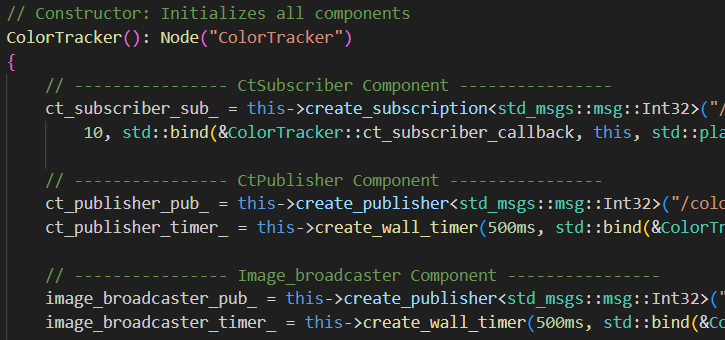
\includegraphics[width=\textwidth]{comments.png}
	\caption{Example of generated code with comments}
	\label{fig:comment}
\end{figure}

Figure~\ref{fig:comment} illustrates how the comments vary depending on the component, this also provides a degree of separation that helps developers understand where parts of the input model are being implemented.

More examples of code comments (with before and after) can be found in the Appendix~\ref{app:comment}.


\subsection{Traceability}
\label{sec:impl_trace}

The implementation of traceability is related with the report feature, however, traceability can exist without a report and a report can exist without traceability~\ref{sec:impl_report}. The main idea of traceability is to relate the coding files directly to the model so we are able to verify that a certain file came from a certain part of the model.

The base construction of the trace file was done in JSON, this provides information while still maintaining a structure that can easily be ported elsewhere.

This is an example of the JSON produced by a traceability analysis:

\begin{verbatim}
{
	"system": "Robot_Vision_I_Instance",
	"generatedAt": "2025-07-28 16:26:49",
	"location": "C:/Users/aurel/git/codegen-config/fr.mem4csd.codegen.config/results",
	"components": {
		"Usb_Cam_Nd": {
			"file": "robot_vision_i_instance/src/Usb_Cam_Nd_process.cpp",
			"type": "process",
			"subcomponent": [
			{
				"name": "Image_Broadcaster",
				"qualifiedName": "Robot_Vision_I_Instance::Usb_Cam_Nd::Image_Broadcaster",
				"codeTrace": "@trace name='Image_Broadcaster'",
				"type": "thread",
				"properties": {
					"Dispatch_Protocol": "",
					"Period": ""
				}
			},
			{
				"name": "UsbSpinner",
				"qualifiedName": "Robot_Vision_I_Instance::Usb_Cam_Nd::UsbSpinner",
				"codeTrace": "@trace name='UsbSpinner'",
				"type": "thread",
				"properties": {
					"Dispatch_Protocol": "",
					"Period": ""
				}
			}
			]
		},(...)
\end{verbatim}

As we can see, it relates the model to the code in various forms, mainly code traces, qualified names, file and package locations. On top of that, it provides additional info that is useful for both developers and end users, developers can easily use this \gls{JSON} as input for various tools (generating an alternate report from the one provided for example) and users can use it to trace parts of the code dedicated to a specific component or subcomponent using a combination of the file locations and the code traces.

In addition to this, traceability links were created using Capra to ensure that the \gls{JSON} file can be directly related to the C++ files using the \textit{@trace} indicative.

\subsection{Report}
\label{sec:impl_report}

The report was implemented with the goal of providing a clear, concise and structured way of visualizing exactly how the model translates to code. To do this, the report is generated in \gls{HTML} using Acceleo. This is important since it overcomes a few constraints, mainly:

\begin{itemize} 
	\item \textbf{PDF with Java:} The major issue that producing \gls{HTML} code with Acceleo instead of a direct PDF with Java fixes is that producing PDFs with Java code, although more practical on the surface, has many limitations when it comes to designing and structuring PDFs. In addition, the verbose is very unintuitive and can quickly grow in complexity.
	\item \textbf{Extensibility:} Since \gls{HTML} is a simple and well known language, adding details and making changes is straightforward when comparing it to other tools like LaTeX. In this case, the usage of LaTeX isn't really justified since it is more directed to academic circumstances and not fast paced development. 
	\item \textbf{Styling Issues:} Using raw \gls{CSS} in combination with \gls{HTML} is no doubt the best choice when it comes to styling the report. Java has many limitations when it comes to styling and LaTeX is very strict and error prone. For a basic report such as the one generated, \gls{CSS} styling is more than enough.
\end{itemize}

Once these constraints were no longer an issue, the development of the report was much more intuitive. The base was made with \gls{HTML} and \gls{CSS}, which enabled a high degree of custom styles while also simplifying the integration of useful information. 

Since the first iteration of the report was done in \gls{HTML}, the transition to PDF was mostly seamless, however, its implementation was done not by Java code, but via Workflow. This was at a later stage, a more detailed explanation can be found in Section~\ref{label}.

The report has many features, its high customization enables the creation of different parts when needed, hence omitting redundant or unwanted sections according to user needs. One of the core elements is the \gls{ROS} specific option, which highlights \gls{ROS} specific components that were generated or ported from the model. This allows \gls{ROS} developers to have a much clearer idea of how parts of the input model were represented in the \gls{ROS} part of the code, for instance, what thread corresponds to a Publisher\footnote{Publishers generate and publish data (sensor readings, etc).} or Subscriber\footnote{Subscribers listen for and process data sent by Publishers.}.









